\documentclass{article}

% NeurIPS 2026 submission style. The default option is the main-track,
% double-blind submission format (line numbers and anonymized author block).
\usepackage{neurips_2026}

\usepackage[utf8]{inputenc}
\usepackage[T1]{fontenc}
\usepackage{hyperref}
\usepackage{url}
\usepackage{booktabs}
\usepackage{amsmath}
\usepackage{amssymb}
\usepackage{nicefrac}
\usepackage{microtype}
\usepackage{xcolor}
\usepackage{graphicx}
\usepackage{tikz}
\usetikzlibrary{arrows.meta,positioning,calc}

\title{Evaluating Sparse Dynamical Regularization for Financial Forecasting under Market Regime Shifts}

\author{%
  Anonymous Author(s) \\
  CSC413 Course Project Proposal \\
  \texttt{anonymous@example.edu}
}

\begin{document}

\maketitle

\begin{abstract}
Financial time series are nonstationary: return predictability, volatility, and cross-asset dependence can change abruptly when the market enters a new regime. We propose a controlled study of \emph{sparse dynamical regularization} for multi-asset financial forecasting under such shifts. The proposed model encodes a lookback window of asset and macro-financial features into a low-dimensional latent state, infers a causal mixture of market regimes, and constrains the latent state to evolve according to a small set of reusable SINDy-style dynamical terms with regime-specific coefficients. A forecast head outputs next-day return distributions. The central question is not whether a larger recurrent network can fit historical returns, but whether a sparse dynamical prior improves out-of-distribution performance when volatility, correlations, and macro conditions change. We will compare the model against dense recurrent networks, generic regularization, capacity-matched controls, neural-ODE forecasting, and SINDy-SHRED variants on a 2005--2025 U.S. ETF panel using rolling-origin backtests. Evaluation will combine regime-stratified accuracy and calibration, trading-relevant metrics, and stability of the discovered dynamical terms. The project will therefore test whether sparsity is a useful inductive bias for regime-shift robustness, rather than merely a source of reduced model capacity.
\end{abstract}

\section{Introduction}

Financial forecasting is a canonical nonstationary time-series problem. The joint distribution of returns, volatility, and correlations is not fixed: the 2008 financial crisis, the 2020 COVID-19 shock, the 2022 inflation and rate-hiking cycle, and the 2023 regional-banking stress produced different market dynamics from the calm periods around them. A model trained on one regime can exploit correlations that disappear in another, and high-capacity sequence models can memorize regime-specific noise. This makes financial forecasting a particularly informative test bed for regularization methods that encode structural assumptions about temporal dynamics.

Deep learning is attractive here because financial panels contain high-dimensional, nonlinear, cross-asset dependencies that are difficult to specify by hand. However, standard recurrent models are flexible precisely because they impose few restrictions on the latent transition. Weight decay, dropout, and early stopping reduce variance, but they do not encode the hypothesis that market dynamics are generated by a small number of interpretable mechanisms. Sparse identification of nonlinear dynamics (SINDy) offers a different prior: the state derivative is a linear combination of a library of candidate terms, and an $\ell_1$-type penalty selects a parsimonious subset \citep{brunton2016}. When combined with a learned encoder, this prior can be applied to noisy, partially observed data \citep{champion2019,gao2026sindyshred}. Whether the prior actually helps under market regime shifts, however, is an empirical question that existing work has not answered systematically.

\paragraph{Problem statement and input--output format.}
Let $t$ index trading days and let $N$ be the number of assets. At each day $t$, the model receives (i) a lookback window
\begin{equation}
  X_t = [x_{t-L+1}, \ldots, x_t] \in \mathbb{R}^{L \times d_x},
\end{equation}
where $x_s$ contains lagged asset returns, realized volatilities, volume and range features, and macro-financial variables; and (ii) a causal regime descriptor $r_t \in \mathbb{R}^{d_r}$ constructed only from information available at or before $t$ (for example, VIX percentile, drawdown, term-spread changes, and credit-spread changes). It outputs a predictive distribution for the next-day cross-section of log returns,
\begin{equation}
  p_\theta(Y_t \mid X_t, r_t), \qquad
  Y_t = \left(y_{t+1}^{(1)}, \ldots, y_{t+1}^{(N)}\right) \in \mathbb{R}^{N},
\end{equation}
parameterized by means $\mu_t \in \mathbb{R}^{N}$ and log standard deviations $\log \sigma_t \in \mathbb{R}^{N}$. The primary target is the next-day close-to-close log return; we will additionally report volatility and calibration diagnostics. The model is trained only on data before each test period, and all preprocessing statistics are estimated on the training fold.

\paragraph{Why a dynamical deep-learning approach is reasonable.}
A purely linear model cannot capture nonlinear interactions among volatility, momentum, and cross-asset dependence, while an unrestricted recurrent network may overfit the training regime. Our approach keeps the representational power of a neural encoder but places a structured prior on its latent evolution: the encoder handles high-dimensional observations, and the sparse dynamical layer models how the latent state changes over time. This is a reasonable compromise for financial data because it reduces the effective hypothesis class without assuming that returns themselves follow a simple low-order autoregression.

\paragraph{Contributions.}
This project is an evaluation-first study with three components.
\begin{enumerate}
  \item \textbf{A controlled regime-shift benchmark.} We build a leakage-controlled, rolling-origin evaluation protocol on a liquid U.S. ETF panel and compare models inside and outside known stress windows.
  \item \textbf{A regime-conditioned sparse latent dynamics model.} We extend a SINDy-style latent regularizer with a causal mixture of regime-specific coefficient matrices. Active library terms are shared across regimes through a group-sparse penalty, while their coefficients may differ by regime.
  \item \textbf{Mechanism-focused ablations.} We use capacity-matched dense models, random sparse masks, generic weight penalties, and smoothness-only controls to test whether any improvement is attributable to sparsity itself rather than to fewer parameters or smoother predictions.
\end{enumerate}

\section{Background and Related Work}

\paragraph{SINDy and sparse dynamical models.}
SINDy assumes that a state $x(t)$ evolves according to
\begin{equation}
  \dot{x}(t) = \Theta(x(t))^\top \xi,
\end{equation}
where $\Theta(x)$ is a library of candidate functions (constant, polynomial, and interaction terms) and $\xi$ is a sparse coefficient vector. The coefficients are estimated by sparse regression, so that only a small number of terms are active \citep{brunton2016}. The approach yields interpretable equations when the state is fully observed and the library contains the relevant terms. Financial returns are noisy and only partially observed, so applying SINDy directly in return space is fragile; we instead use it as a regularizer on a learned latent state.

\paragraph{Joint learning of coordinates and dynamics.}
\citet{champion2019} showed that an autoencoder can jointly learn a low-dimensional coordinate system and a sparse dynamical model in that coordinate system. Their method avoids requiring the observed variables to be the natural state variables and demonstrates that SINDy constraints can be imposed end-to-end. Our proposal follows this general idea but focuses on a different question: whether the resulting parsimony improves forecasting when the data-generating process changes across market regimes. We also use a causal encoder rather than an autoencoder over the full sample, which is essential for a valid financial backtest.

\paragraph{SINDy-SHRED and direct precursors.}
The closest work is SINDy-SHRED \citep{gao2026sindyshred}, which combines gated recurrent units (GRUs), a shallow decoder, and SINDy-based regularization of the latent space. It demonstrates that sparse latent dynamics can improve accuracy, data efficiency, and training time in spatio-temporal forecasting, and that restricting the latent dynamics to a linear model yields a Koopman-style model. Our work directly builds on this line: we adapt the idea to a multivariate financial panel and ask whether the same sparse prior remains beneficial under abrupt distribution shift. Unlike SINDy-SHRED, we explicitly condition the coefficient matrices on a causal regime representation and evaluate the model on stress periods that are not represented in training.

\paragraph{Recurrent networks for financial prediction.}
\citet{fischer2018} provide an influential evaluation of LSTM networks for financial market prediction and show that deep sequence models can extract predictive structure from historical price data. Their study motivates the use of recurrent encoders, but it does not impose an explicit dynamical prior and does not isolate robustness to regime change. We use a GRU encoder as the backbone of both our sparse and dense models so that the comparison is not confounded by a different sequence model.

\paragraph{Adaptation under nonstationary markets.}
\citet{wang2026} study meta-learning for return prediction when market regimes shift. Their approach adapts a predictive model across tasks or regimes and is complementary to ours: they focus on how to adapt at the level of learning algorithms, whereas we focus on the structure of the latent dynamics and on whether sparsity improves out-of-distribution generalization. A useful comparison is therefore a meta-learning baseline in addition to standard recurrent baselines.

\paragraph{Continuous-time neural forecasting.}
\citet{nguyen2024} propose a phase-space-reconstructed neural ordinary differential equation model for stock price forecasting. Neural ODEs model continuous-time state evolution and can represent irregular or nonlinear dynamics, but they do not by themselves select a small set of interpretable terms. Our study compares sparse latent dynamics against a neural-ODE forecasting baseline and tests whether the added sparsity prior improves regime-shift performance.

\paragraph{Positioning.}
Table~\ref{tab:related} summarizes the distinctions. The contribution of this project is not a new general-purpose sequence architecture. It is a systematic test of a specific structural prior---sparse latent dynamics with regime-conditioned coefficients---under a protocol designed to separate genuine robustness from capacity reduction. This distinction matters because a sparse model may appear more robust simply because it has fewer parameters or produces smoother forecasts.

\begin{table}[t]
  \caption{Related work and the gap addressed by this proposal. The final row is the proposed model and evaluation setting.}
  \label{tab:related}
  \centering
  \small
  \begin{tabular}{@{}p{3.4cm}p{2.6cm}p{1.6cm}p{3.0cm}@{}}
    \toprule
    Method & Latent dynamics & Sparse prior & Regime adaptation \\
    \midrule
    SINDy (2016) & No (observed) & Yes & No \\
    Champion et al. (2019) & Yes (autoencoder) & Yes & No \\
    SINDy-SHRED (2026) & Yes (GRU decoder) & Yes & No \\
    Fischer \& Krauss (2018) & No explicit prior & No & No \\
    Wang \& Lera (2026) & No explicit prior & No & Meta-learning \\
    Nguyen et al. (2024) & Neural ODE & No & No \\
    \midrule
    Proposed (this work) & Yes & Yes & Causal regime mixture \\
    \bottomrule
  \end{tabular}
\end{table}

\section{Data}

\paragraph{Universe and period.}
We will use a panel of 16 liquid U.S.-listed ETFs from January 2005 through December 2025: SPY, QQQ, IWM, EEM, EFA, TLT, GLD, and the nine original sector SPDRs (XLB, XLE, XLF, XLI, XLK, XLP, XLU, XLV, XLY). This universe spans broad equity, growth, small-cap, international, emerging-market, long-duration bond, gold, and sector exposures. It has long histories, high liquidity, and no need to reconstruct a point-in-time constituent list, which keeps the proposal feasible for a course project. Macro-financial variables are obtained from FRED (VIX, 3-month and 10-year Treasury yields, the BAA--10-year credit spread, and a broad dollar index), and daily ETF prices and volumes are obtained from a public market-data source. We will document the exact retrieval date and data version.

\paragraph{Features.}
For each asset and day, the feature vector includes the one-day log return, 5-day and 20-day realized volatility, 20-day momentum, log dollar volume standardized over a trailing window, and the high--low range. Market-level features include VIX level and percentile, SPY drawdown from its 252-day high, the 10-year minus 3-month term spread and its 20-day change, the credit-spread level and change, and the broad dollar return. All features are computed only from past observations. Returns and volatility are winsorized at the 1st and 99th percentiles using training-fold thresholds, and missing observations are forward-filled only for at most two consecutive days.

\paragraph{Target and regime strata.}
The primary target is the next-day close-to-close log return for each of the 16 ETFs. For evaluation only, we label each test day as \emph{calm}, \emph{transition}, or \emph{stress} using ex post information: stress if VIX exceeds 30 or SPY has fallen more than 10\% from its 60-day high; calm if VIX is below 15 and SPY is above its 200-day moving average; otherwise transition. These labels are never provided to the model. We also report results for the event windows 2008--2009 (global financial crisis), 2011 (euro-area debt stress), 2018 Q4 (equity sell-off), 2020 (COVID-19 shock), 2022 (inflation and rate shock), and 2023 (regional-banking stress). As a robustness check, we will repeat the stratification with a three-state Gaussian hidden Markov model fitted only on training data, so that regime definitions are not tied to hand-chosen thresholds.

\paragraph{Splits and leakage control.}
Model development uses 2005--2017. Hyperparameters are selected by expanding-window validation within this period. The final out-of-sample evaluation uses walk-forward refitting for test years 2018--2025: for test year $y$, the model is trained on all data through the end of year $y-1$ and tested on year $y$ (with a one-year gap only if needed to avoid overlapping labels). No future data are used for scaling, feature construction, early stopping, or regime inference. We will report both pooled test metrics and metrics conditional on the ex post regime labels. The main exploratory diagnostics will be (i) regime frequencies and event durations, (ii) autocorrelation and volatility clustering, and (iii) cross-asset correlation in calm versus stress periods; these diagnostics motivate the lookback length and latent dimension.

\paragraph{Exploratory diagnostic.}
Figure~\ref{fig:vix} shows the monthly average CBOE VIX over the sample and marks the stress periods used for evaluation. The series displays strong volatility clustering and several abrupt regime changes, which motivates our focus on out-of-distribution performance rather than only average-case accuracy. We will add analogous plots for cross-asset correlation and feature distributions in the final report.

\begin{figure}[t]
  \centering
  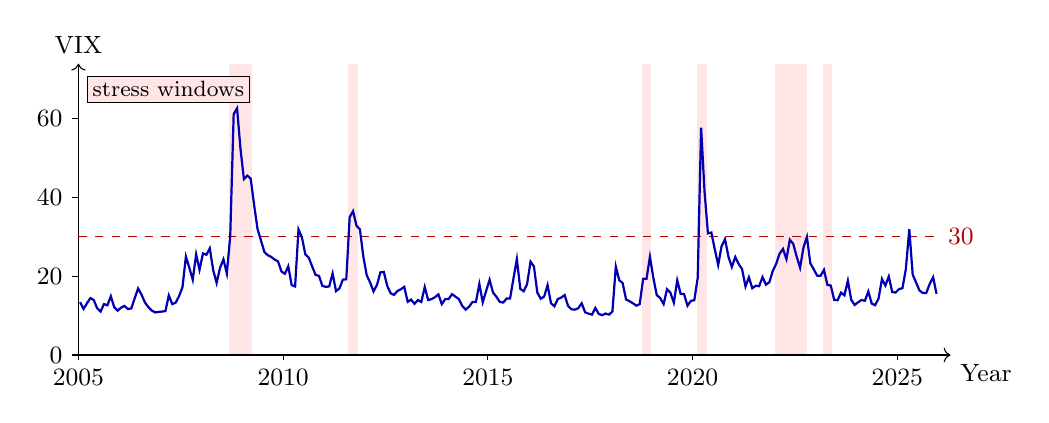
\begin{tikzpicture}[x=0.52cm,y=0.05cm,font=\small]
    % Shaded event windows are used only for evaluation.
    \fill[red!10] (3.67,0) rectangle (4.25,74);
    \fill[red!10] (6.59,0) rectangle (6.82,74);
    \fill[red!10] (13.76,0) rectangle (13.99,74);
    \fill[red!10] (15.10,0) rectangle (15.34,74);
    \fill[red!10] (17.02,0) rectangle (17.80,74);
    \fill[red!10] (18.19,0) rectangle (18.40,74);

    \draw[->] (0,0) -- (21.3,0) node[below right] {Year};
    \draw[->] (0,0) -- (0,74) node[above] {VIX};
    \foreach \y in {0,20,40,60} \draw (0,\y) -- (-0.15,\y) node[left] {\y};
    \foreach \x/\yr in {0/2005,5/2010,10/2015,15/2020,20/2025}
      \draw (\x,0) -- (\x,-1.3) node[below] {\yr};
    \draw[dashed, red!70!black] (0,30) -- (21.0,30) node[right] {30};
      \draw[blue!70!black, thick] plot coordinates { (0.042,13.44) (0.125,11.71) (0.208,13.13) (0.292,14.46)
     (0.375,13.97) (0.458,11.87) (0.542,11.05) (0.625,12.95) (0.708,12.63) (0.792,14.94) (0.875,12.15)
     (0.958,11.26) (1.042,12.04) (1.125,12.47) (1.208,11.69) (1.292,11.85) (1.375,14.45) (1.458,16.92)
     (1.542,15.33) (1.625,13.35) (1.708,12.18) (1.792,11.31) (1.875,10.82) (1.958,10.96) (2.042,11.04)
     (2.125,11.16) (2.208,15.16) (2.292,12.93) (2.375,13.30) (2.458,14.95) (2.542,17.27) (2.625,25.03)
     (2.708,22.20) (2.792,19.12) (2.875,25.58) (2.958,21.65) (3.042,25.82) (3.125,25.46) (3.208,27.10)
     (3.292,21.56) (3.375,18.30) (3.458,22.11) (3.542,24.32) (3.625,20.70) (3.708,30.24) (3.792,61.18)
     (3.875,62.67) (3.958,52.41) (4.042,44.68) (4.125,45.57) (4.208,44.80) (4.292,38.06) (4.375,31.98)
     (4.458,29.14) (4.542,26.16) (4.625,25.34) (4.708,24.93) (4.792,24.25) (4.875,23.79) (4.958,21.24)
     (5.042,20.64) (5.125,22.54) (5.208,17.77) (5.292,17.42) (5.375,31.93) (5.458,29.92) (5.542,25.57)
     (5.625,24.75) (5.708,22.52) (5.792,20.37) (5.875,20.10) (5.958,17.57) (6.042,17.32) (6.125,17.43)
     (6.208,20.72) (6.292,16.24) (6.375,16.91) (6.458,19.15) (6.542,19.23) (6.625,35.03) (6.708,36.53)
     (6.792,32.83) (6.875,31.94) (6.958,25.05) (7.042,20.23) (7.125,18.42) (7.208,16.17) (7.292,17.82)
     (7.375,21.00) (7.458,21.13) (7.542,17.57) (7.625,15.69) (7.708,15.28) (7.792,16.28) (7.875,16.70)
     (7.958,17.31) (8.042,13.51) (8.125,14.07) (8.208,13.03) (8.292,13.97) (8.375,13.49) (8.458,17.27)
     (8.542,13.97) (8.625,14.21) (8.708,14.69) (8.792,15.41) (8.875,12.92) (8.958,14.19) (9.042,14.24)
     (9.125,15.47) (9.208,14.84) (9.292,14.20) (9.375,12.48) (9.458,11.54) (9.542,12.30) (9.625,13.49)
     (9.708,13.47) (9.792,18.06) (9.875,13.41) (9.958,16.29) (10.042,19.12) (10.125,15.90) (10.208,14.81)
     (10.292,13.49) (10.375,13.34) (10.458,14.34) (10.542,14.35) (10.625,19.43) (10.708,24.38) (10.792,16.79)
     (10.875,16.21) (10.958,18.03) (11.042,23.72) (11.125,22.52) (11.208,15.85) (11.292,14.30) (11.375,14.85)
     (11.458,17.77) (11.542,13.16) (11.625,12.40) (11.708,14.22) (11.792,14.59) (11.875,15.24) (11.958,12.47)
     (12.042,11.61) (12.125,11.53) (12.208,11.90) (12.292,13.14) (12.375,10.86) (12.458,10.51) (12.542,10.26)
     (12.625,11.98) (12.708,10.44) (12.792,10.13) (12.875,10.54) (12.958,10.26) (13.042,11.06) (13.125,22.46)
     (13.208,19.02) (13.292,18.27) (13.375,14.12) (13.458,13.68) (13.542,13.15) (13.625,12.55) (13.708,12.91)
     (13.792,19.35) (13.875,19.39) (13.958,24.95) (14.042,19.57) (14.125,15.23) (14.208,14.49) (14.292,12.95)
     (14.375,16.72) (14.458,15.84) (14.542,13.31) (14.625,18.98) (14.708,15.56) (14.792,15.47) (14.875,12.52)
     (14.958,13.76) (15.042,13.94) (15.125,19.63) (15.208,57.74) (15.292,41.45) (15.375,30.90) (15.458,31.12)
     (15.542,26.84) (15.625,22.89) (15.708,27.65) (15.792,29.44) (15.875,25.00) (15.958,22.37) (16.042,24.91)
     (16.125,23.14) (16.208,21.84) (16.292,17.42) (16.375,19.76) (16.458,16.96) (16.542,17.60) (16.625,17.47)
     (16.708,19.82) (16.792,17.87) (16.875,18.50) (16.958,21.35) (17.042,23.18) (17.125,25.75) (17.208,26.97)
     (17.292,24.37) (17.375,29.31) (17.458,28.23) (17.542,25.00) (17.625,22.17) (17.708,27.34) (17.792,30.01)
     (17.875,23.30) (17.958,21.78) (18.042,20.17) (18.125,20.12) (18.208,21.64) (18.292,17.82) (18.375,17.64)
     (18.458,14.00) (18.542,13.93) (18.625,15.85) (18.708,15.17) (18.792,18.89) (18.875,14.02) (18.958,12.72)
     (19.042,13.39) (19.125,13.98) (19.208,13.79) (19.292,16.14) (19.375,13.06) (19.458,12.67) (19.542,14.37)
     (19.625,19.31) (19.708,17.66) (19.792,19.96) (19.875,16.02) (19.958,15.87) (20.042,16.76) (20.125,16.97)
     (20.208,21.84) (20.292,31.97) (20.375,20.46) (20.458,18.40) (20.542,16.38) (20.625,15.75) (20.708,15.79)
     (20.792,18.09) (20.875,19.77) (20.958,15.55) };
    \node[draw, fill=red!10, inner sep=2pt, font=\footnotesize, anchor=north west] at (0.2,71) {stress windows};
  \end{tikzpicture}
  \caption{Monthly average CBOE VIX over the proposed sample (FRED series VIXCLS, January 2005--December 2025). Shaded bands mark the stress windows used in the evaluation: the global financial crisis, the 2011 euro-area debt stress, 2018 Q4, the COVID-19 shock, the 2022 inflation and rate shock, and the 2023 regional-banking stress. The figure illustrates volatility clustering and abrupt regime changes; the stress labels are used only for evaluation and are never provided to the model.}
  \label{fig:vix}
\end{figure}

\section{Model Architecture}

\paragraph{Overview.}
We propose a Sparse Regime-Conditioned Dynamics model (SRCD). It consists of four modules: a causal sequence encoder, a regime encoder, a regime-conditioned sparse latent dynamics layer, and a distributional forecast head. A shallow decoder is used only as an auxiliary reconstruction pathway that prevents the latent state from discarding information needed by the dynamics model. Figure~\ref{fig:architecture} gives an overview.

\paragraph{Encoder.}
A one-layer GRU with 64 hidden units processes the standardized window $X_t$ and produces a hidden state $h_t$. A linear layer maps $h_t$ to an $m$-dimensional latent state $z_t \in \mathbb{R}^{m}$ with $m=8$ in the main experiments. Layer normalization and dropout ($p=0.1$) are applied to stabilize training. The encoder is shared by all assets, while the forecast head produces an asset-specific output vector.

\paragraph{Causal regime encoder.}
A small multilayer perceptron $g_\phi$ maps the regime descriptor $r_t$ to $K$ logits and then to regime weights
\begin{equation}
  \pi_t = \mathrm{softmax}(g_\phi(r_t)) \in \Delta^{K-1},
\end{equation}
where $K=3$ in the main experiments. The descriptor contains only causal transformations of past market variables. We emphasize that $\pi_t$ is an inferred soft regime assignment, not a ground-truth label; the ex post labels are used only for evaluation.

\paragraph{Sparse regime-conditioned latent dynamics.}
Let $\Theta(z_t) \in \mathbb{R}^{1 \times p}$ be a library containing a constant, linear terms, and all quadratic monomials of $z_t$ (plus a small number of interactions if the latent dimension is increased). Each regime $k$ has a coefficient matrix $\Xi_k \in \mathbb{R}^{p \times m}$. The effective dynamics are a convex mixture:
\begin{equation}
  \Xi_t = \sum_{k=1}^{K} \pi_{t,k} \Xi_k,
  \qquad
  \hat{z}_{t+1} = z_t + \Delta\, \Theta(z_t)^\top \Xi_t,
  \label{eq:dynamics}
\end{equation}
where $\Delta$ is a fixed one-trading-day step (or a learned positive scalar). The one-step latent prediction $\hat{z}_{t+1}$ is trained to match the encoding of the next observation, $z_{t+1}=f_\theta(X_{t+1})$. This is an Euler discretization of a continuous-time SINDy model; it retains the linear-in-parameters structure that makes sparse regression possible while allowing the neural encoder to learn the latent coordinates.

\paragraph{Sparse penalty.}
To encourage a small set of dynamical mechanisms, we use a shared-support group penalty
\begin{equation}
  \Omega_{\mathrm{sparse}}(\Xi)
  = \sum_{j=1}^{p}
    \left(
      \sum_{k=1}^{K} \left\| \Xi_k[j,:] \right\|_2^2
    \right)^{1/2}.
  \label{eq:sparse}
\end{equation}
For a given library term $j$, the penalty is zero only if that term is inactive in every regime; if the term is active, its coefficient may still differ across regimes. This structure matches the scientific question: we want to discover a small set of reusable mechanisms, while allowing their strengths to change with market conditions. An ablation replaces \eqref{eq:sparse} with independent $\ell_1$ penalties on each $\Xi_k$, and another removes the regime conditioning entirely ($K=1$).

\paragraph{Forecast head and auxiliary decoder.}
The forecast head $h_\psi$ maps the concatenation $[z_t, \pi_t, r_t]$ to $2N$ outputs, interpreted as means and log standard deviations:
\begin{equation}
  (\mu_t, \log \sigma_t) = h_\psi(z_t, \pi_t, r_t).
\end{equation}
The predictive loss is the Gaussian negative log-likelihood
\begin{equation}
  \mathcal{L}_{\mathrm{pred}}
  = \frac{1}{N}\sum_{i=1}^{N}
    \left[
      \frac{(y_{t+1}^{(i)}-\mu_{t,i})^2}{2\sigma_{t,i}^2}
      + \log \sigma_{t,i}
    \right].
\end{equation}
A shallow decoder $D_\omega$ reconstructs the final observation $x_t$ from $z_t$ with mean-squared error $\mathcal{L}_{\mathrm{rec}}$. This auxiliary pathway stabilizes the latent representation and discourages a degenerate solution in which the encoder maps all inputs to an almost constant state. The dynamics loss is
\begin{equation}
  \mathcal{L}_{\mathrm{dyn}}
  = \left\| z_{t+1} - \hat{z}_{t+1} \right\|_2^2.
\end{equation}
The total objective is
\begin{equation}
  \mathcal{L}
  = \mathcal{L}_{\mathrm{pred}}
  + \lambda_r \mathcal{L}_{\mathrm{rec}}
  + \lambda_d \mathcal{L}_{\mathrm{dyn}}
  + \lambda_s \Omega_{\mathrm{sparse}}(\Xi)
  + \lambda_w \|\theta\|_2^2,
  \label{eq:total-loss}
\end{equation}
where $\lambda_r,\lambda_d,\lambda_s,\lambda_w$ are selected on validation data.

\paragraph{Training details.}
We use AdamW with learning rate $10^{-3}$, weight decay $10^{-4}$, batch size 64, gradient clipping at norm 1.0, and early stopping with patience 10 on a regime-balanced validation loss. The maximum number of epochs is 100. The sparsity weight $\lambda_s$ is selected from $\{10^{-4},10^{-3},10^{-2},10^{-1}\}$; $\lambda_d$ from $\{0.01,0.1,1\}$; and $\lambda_r$ from $\{0.01,0.1,1\}$. All models are trained with five random seeds. The encoder and forecast head are identical across the sparse and dense variants, so differences in performance can be attributed to the dynamics prior rather than to a different feature extractor.

\subsection{Architecture Figure}

Figure~\ref{fig:architecture} was created for this proposal and shows the complete computation graph, including the causal data path, the regime path, and the training signals. The diagram is modular: the dense, static-sparse, and regime-conditioned variants are obtained by removing the corresponding components while keeping the encoder and forecast head unchanged.

\begin{figure}[t]
  \centering
  \resizebox{\linewidth}{!}{%
  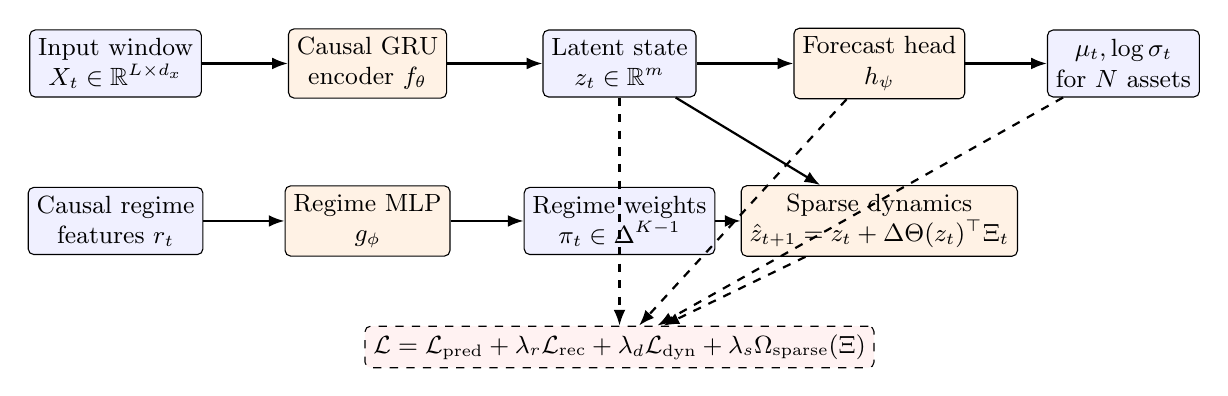
\begin{tikzpicture}[
    font=\small,
    box/.style={draw, rounded corners=2pt, align=center, minimum height=0.85cm, inner sep=3pt},
    data/.style={box, fill=blue!6},
    op/.style={box, fill=orange!10},
    loss/.style={draw, dashed, rounded corners=2pt, fill=red!5, align=center, inner sep=3pt},
    arr/.style={-{Latex[length=2mm]}, thick},
    darr/.style={-{Latex[length=2mm]}, dashed, thick}
  ]
    \node[data] (x) at (0,2.2) {Input window\\$X_t\in\mathbb{R}^{L\times d_x}$};
    \node[op]   (enc) at (3.2,2.2) {Causal GRU\\encoder $f_\theta$};
    \node[data] (z) at (6.4,2.2) {Latent state\\$z_t\in\mathbb{R}^{m}$};
    \node[op]   (head) at (9.7,2.2) {Forecast head\\$h_\psi$};
    \node[data] (out) at (12.8,2.2) {$\mu_t,\log\sigma_t$\\for $N$ assets};

    \node[data] (r) at (0,0.2) {Causal regime\\features $r_t$};
    \node[op]   (reg) at (3.2,0.2) {Regime MLP\\$g_\phi$};
    \node[data] (pi) at (6.4,0.2) {Regime weights\\$\pi_t\in\Delta^{K-1}$};
    \node[op]   (dyn) at (9.7,0.2) {Sparse dynamics\\$\hat z_{t+1}=z_t+\Delta\Theta(z_t)^\top\Xi_t$};

    \node[loss] (loss) at (6.4,-1.4) {$\mathcal{L}=\mathcal{L}_{\mathrm{pred}}+\lambda_r\mathcal{L}_{\mathrm{rec}}+\lambda_d\mathcal{L}_{\mathrm{dyn}}+\lambda_s\Omega_{\mathrm{sparse}}(\Xi)$};

    \draw[arr] (x) -- (enc);
    \draw[arr] (enc) -- (z);
    \draw[arr] (z) -- (head);
    \draw[arr] (head) -- (out);
    \draw[arr] (r) -- (reg);
    \draw[arr] (reg) -- (pi);
    \draw[arr] (pi) -- (dyn);
    \draw[arr] (z) -- (dyn);
    \draw[darr] (z) -- (loss);
    \draw[darr] (dyn) -- (loss);
    \draw[darr] (head) -- (loss);
    \draw[darr] (out) -- (loss);
  \end{tikzpicture}%
  }
  \caption{Overview of the proposed Sparse Regime-Conditioned Dynamics model. A causal GRU encodes a multivariate window into a low-dimensional latent state. A separate regime encoder produces soft regime weights that modulate a mixture of sparse SINDy coefficient matrices. The latent state feeds both the forecast head and the sparse one-step dynamics loss; an auxiliary decoder and a shared-support sparsity penalty regularize the latent representation and the discovered terms. The ex post regime labels used for evaluation are never model inputs.}
  \label{fig:architecture}
\end{figure}

\section{Proposed Evaluation and Ablations}

\paragraph{Hypotheses.}
We will test three pre-specified hypotheses. \textbf{H1 (robustness):} sparse latent dynamics reduce worst-regime forecast error and calibration loss relative to dense GRU and weight-decay controls, after matching parameter count. \textbf{H2 (adaptivity):} regime-conditioned coefficients improve performance when the regime descriptor changes, but not necessarily in calm periods; the benefit should be largest for stress-to-calm or calm-to-stress transitions. \textbf{H3 (interpretability):} the active library terms are stable across rolling refits and their coefficient changes align with known market shifts. A negative result is informative: if gains disappear after capacity matching and smoothness controls, we will conclude that the apparent benefit of sparsity comes from generic regularization rather than from a sparse dynamical mechanism.

\paragraph{Baselines.}
We will compare the full model with: (i) an unconditional historical-mean forecast; (ii) ridge regression on lagged features; (iii) a GRU with the same encoder and forecast head but no dynamics loss; (iv) the same GRU with dropout and weight decay; (v) a dense latent-dynamics model with $\lambda_s=0$; (vi) a static sparse SINDy model with $K=1$; (vii) a neural-ODE forecasting model in the spirit of \citet{nguyen2024}; and (viii) a SINDy-SHRED-style model adapted to the ETF panel. The GRU-based models share the same input pipeline and forecast head to make comparisons as controlled as possible.

\paragraph{Ablations.}
The main ablation varies the sparsity weight $\lambda_s$ over a logarithmic grid and reports the full sparsity--performance frontier. To test whether sparsity itself matters, we include (a) a random sparse mask with the same number of active terms as the learned model, (b) an $\ell_1$ penalty on the GRU weights, (c) a temporal-smoothness penalty on latent states with no sparsity, and (d) a reduced-capacity GRU whose parameter count matches the sparse model. We also compare $K=1$, $K=3$, and an oracle-regime upper bound that uses ex post labels only for diagnosis (never as a deployable model). Finally, we vary the latent dimension $m\in\{4,8,16\}$ and the lookback $L\in\{20,60,120\}$ to check whether the conclusions are sensitive to capacity and memory.

\paragraph{Metrics.}
Forecast quality will be measured by mean squared error, mean absolute error, out-of-sample $R^2$, Spearman information coefficient, directional accuracy, Gaussian negative log-likelihood, and continuous ranked probability score. Because financial forecasts are often used in portfolio construction, we will also report a simple long--short portfolio Sharpe ratio and turnover after a conservative transaction-cost assumption. Regime-robustness will be summarized by regime-stratified metrics, the worst-regime score, and the ratio of stress-period to calm-period error. Calibration will be assessed with 90\% interval coverage and reliability plots. Interpretability will be assessed by the number of active library terms, support stability across folds (Jaccard similarity), and coefficient drift across regimes and time.

\paragraph{Statistical protocol.}
All results will be averaged over five seeds and reported with standard deviations. Differences between the proposed model and each baseline will be tested using Diebold--Mariano tests for forecast errors and a moving-block bootstrap for trading metrics, with blocks chosen to preserve serial dependence. Because the test period contains only a small number of major regimes, we will interpret event-level results descriptively and avoid claiming statistical significance from a single crisis window. We will release the code, preprocessing scripts, data manifest, and selected model coefficients with the final report.

\section{Ethical Considerations}

This project uses public market data and does not involve human subjects or personally identifiable information. The main ethical risk is that a plausible-looking financial forecasting model may be interpreted as investment advice or as evidence of a profitable trading strategy. Backtests are necessarily simplified: they ignore market impact, capacity limits, borrow costs, and some execution frictions, and they can overstate performance through survivorship or selection effects. We will therefore present the work as a methodological study, not as a deployable trading system, and will report uncertainty, out-of-sample results, and the assumptions behind any portfolio metric.

A second risk is overclaiming interpretability. Sparse latent terms are predictive associations in a learned coordinate system, not discovered laws of markets, and coefficient changes under regime shift may reflect confounding rather than causal mechanisms. We will avoid causal language and will clearly label the regime labels and sparse supports as model-dependent constructs. Because financial models can be used to concentrate risk or to exploit other market participants, we will not release a live-trading interface and will include a clear warning about misuse. Finally, the compute footprint is modest---the models are small enough to train on a single GPU---and we will document data licenses and random seeds so that the results can be audited and reproduced.

\begin{thebibliography}{9}
\small

\bibitem[Brunton et al.(2016)]{brunton2016}
S.~L. Brunton, J.~L. Proctor, and J.~N. Kutz.
\newblock Discovering governing equations from data by sparse identification of nonlinear dynamical systems.
\newblock \emph{Proceedings of the National Academy of Sciences}, 113(15):3932--3937, 2016.
\newblock DOI: 10.1073/pnas.1517384113.

\bibitem[Champion et al.(2019)]{champion2019}
K.~Champion, B.~Lusch, J.~N. Kutz, and S.~L. Brunton.
\newblock Data-driven discovery of coordinates and governing equations.
\newblock \emph{Proceedings of the National Academy of Sciences}, 116(45):22445--22451, 2019.
\newblock DOI: 10.1073/pnas.1906995116.

\bibitem[Gao et al.(2026)]{gao2026sindyshred}
M.~L. Gao, J.~P. Williams, and J.~N. Kutz.
\newblock Sparse identification of nonlinear dynamics and Koopman operators with Shallow Recurrent Decoder Networks.
\newblock \emph{Proceedings of the National Academy of Sciences}, 123(16):e2508144123, 2026.
\newblock DOI: 10.1073/pnas.2508144123.

\bibitem[Fischer and Krauss(2018)]{fischer2018}
T.~Fischer and C.~Krauss.
\newblock Deep learning with long short-term memory networks for financial market predictions.
\newblock \emph{European Journal of Operational Research}, 270(2):654--669, 2018.
\newblock DOI: 10.1016/j.ejor.2017.11.054.

\bibitem[Wang and Lera(2026)]{wang2026}
Y.~Wang and S.~C. Lera.
\newblock Meta-learning for return prediction in shifting market regimes.
\newblock \emph{Journal of Financial Markets}, 79:101042, 2026.
\newblock DOI: 10.1016/j.finmar.2025.101042.

\bibitem[Nguyen et al.(2024)]{nguyen2024}
A.~Q. Nguyen, S.~Ha, and H.~Thai.
\newblock Phase space reconstructed neural ordinary differential equations model for stock price forecasting.
\newblock In \emph{Proceedings of the Pacific Asia Conference on Information Systems (PACIS)}, 2024.

\end{thebibliography}

\end{document}
